\section{The sixteen-cell five-observable measurement}
\label{sec:fived16}
% DECISION-20261027-joseph-5d-integration-then-second-scope-review.md item 2. Every number is \fvval{key} from values_fived16.tex, which make_values_fived16.py generates from the readouts it pins by sha256 (S1, CRESP, F0, F0b, G, G-DIAG, G-FOLLOWUP, G-SENS2 and the H2 definition). The readouts are NOT CITABLE FOR an interpretation, coverage or a claim; this section reports their numbers, each beside its matrix.

This section gives a five-dimensional cross-section result with total uncertainties: the data result of configuration~(e) (\S\ref{sec:method-config}) on 16 cells, R00--R15, with the reported covariance $C_{\mathrm{total}}+C_{\mathrm{resp}}$. It is a separate product from the configuration-(a) five-dimensional central value of Secs.~\ref{sec:eavailw} and~\ref{sec:5d} and from the five-axis covariance used with that central value (\S\ref{sec:eavailw-adopted}). Statements in those sections about that central value and that covariance do not describe this result, and statements here do not describe them. The section gives the cells and the result (\S\ref{sec:fived16-result}), the covariance and what it is built from (\S\ref{sec:fived16-cov}), the fake-data tests of the estimator's bias against the covariance (\S\ref{sec:fived16-fd}) and the comparison with generator predictions (\S\ref{sec:fived16-gen}).

\subsection{Cells and result}
\label{sec:fived16-result}
The cells are formed from the H2 grid of \S\ref{sec:gbdt-model-dependence}, which divides each axis once into \fvval{h2-nboxes} boxes, with edges $\pT=(\fvval{h2-edges-pt})$, $\pPar=(\fvval{h2-edges-pz})$, $\Eavail=(\fvval{h2-edges-eavail})$, $q_3=(\fvval{h2-edges-q3})$ and $W=(\fvval{h2-edges-W})$, in the units of App.~\ref{sec:gbdt-diagnostic-definitions}. Of these, \fvval{h2-nsupported} meet that appendix's support rule (minimum expected signal and truth weight). Each supported box with purity below $\tau=\fvval{h2-tau}$ is merged into a neighbour, in \fvval{h2-nmerge} predefined steps. The merges absorb \fvval{h2-nabsorbed} unsupported box into cell R09; the other \fvval{h2-nunreported} are not reported. Each of the 16 resulting cells meets the support rule. Table~\ref{tab:fived16-cells} gives each cell's box, its cell-integrated cross section $f$ and its relative uncertainty.

\begin{table}[htbp]
\centering\footnotesize
\caption{The sixteen reported cells: boxes ($\pT$, $\pPar$ and $q_3$ in GeV/$c$; $\Eavail$ and $W$ in GeV), cell-integrated cross section $f$ in units of $\fvval{f-unit}\,\si{cm^2/nucleon}$, and per-cell relative $\sigma$ (\%) under $C_{\mathrm{total}}$, under $C_{\mathrm{resp}}$ alone and under the reported $C_{\mathrm{total}}+C_{\mathrm{resp}}$ (\S\ref{sec:fived16-cov}).}
\label{tab:fived16-cells}
\begin{tabular}{@{}lcccccrrrr@{}}
\toprule
cell & $\pT$ & $\pPar$ & $\Eavail$ & $q_3$ & $W$ & $f$ & $C_{\mathrm{total}}$ & $C_{\mathrm{resp}}$ & $C_{\mathrm{total}}+C_{\mathrm{resp}}$ \\
\midrule
R00 & \fvval{box-R00-pt} & \fvval{box-R00-pz} & \fvval{box-R00-eavail} & \fvval{box-R00-q3} & \fvval{box-R00-W} & \fvval{f-R00} & \fvval{sig-C_total-R00} & \fvval{sig-C_resp-R00} & \fvval{sig-C_total_resp-R00} \\
R01 & \fvval{box-R01-pt} & \fvval{box-R01-pz} & \fvval{box-R01-eavail} & \fvval{box-R01-q3} & \fvval{box-R01-W} & \fvval{f-R01} & \fvval{sig-C_total-R01} & \fvval{sig-C_resp-R01} & \fvval{sig-C_total_resp-R01} \\
R02 & \fvval{box-R02-pt} & \fvval{box-R02-pz} & \fvval{box-R02-eavail} & \fvval{box-R02-q3} & \fvval{box-R02-W} & \fvval{f-R02} & \fvval{sig-C_total-R02} & \fvval{sig-C_resp-R02} & \fvval{sig-C_total_resp-R02} \\
R03 & \fvval{box-R03-pt} & \fvval{box-R03-pz} & \fvval{box-R03-eavail} & \fvval{box-R03-q3} & \fvval{box-R03-W} & \fvval{f-R03} & \fvval{sig-C_total-R03} & \fvval{sig-C_resp-R03} & \fvval{sig-C_total_resp-R03} \\
R04 & \fvval{box-R04-pt} & \fvval{box-R04-pz} & \fvval{box-R04-eavail} & \fvval{box-R04-q3} & \fvval{box-R04-W} & \fvval{f-R04} & \fvval{sig-C_total-R04} & \fvval{sig-C_resp-R04} & \fvval{sig-C_total_resp-R04} \\
R05 & \fvval{box-R05-pt} & \fvval{box-R05-pz} & \fvval{box-R05-eavail} & \fvval{box-R05-q3} & \fvval{box-R05-W} & \fvval{f-R05} & \fvval{sig-C_total-R05} & \fvval{sig-C_resp-R05} & \fvval{sig-C_total_resp-R05} \\
R06 & \fvval{box-R06-pt} & \fvval{box-R06-pz} & \fvval{box-R06-eavail} & \fvval{box-R06-q3} & \fvval{box-R06-W} & \fvval{f-R06} & \fvval{sig-C_total-R06} & \fvval{sig-C_resp-R06} & \fvval{sig-C_total_resp-R06} \\
R07 & \fvval{box-R07-pt} & \fvval{box-R07-pz} & \fvval{box-R07-eavail} & \fvval{box-R07-q3} & \fvval{box-R07-W} & \fvval{f-R07} & \fvval{sig-C_total-R07} & \fvval{sig-C_resp-R07} & \fvval{sig-C_total_resp-R07} \\
R08 & \fvval{box-R08-pt} & \fvval{box-R08-pz} & \fvval{box-R08-eavail} & \fvval{box-R08-q3} & \fvval{box-R08-W} & \fvval{f-R08} & \fvval{sig-C_total-R08} & \fvval{sig-C_resp-R08} & \fvval{sig-C_total_resp-R08} \\
R09 & \fvval{box-R09-pt} & \fvval{box-R09-pz} & \fvval{box-R09-eavail} & \fvval{box-R09-q3} & \fvval{box-R09-W} & \fvval{f-R09} & \fvval{sig-C_total-R09} & \fvval{sig-C_resp-R09} & \fvval{sig-C_total_resp-R09} \\
R10 & \fvval{box-R10-pt} & \fvval{box-R10-pz} & \fvval{box-R10-eavail} & \fvval{box-R10-q3} & \fvval{box-R10-W} & \fvval{f-R10} & \fvval{sig-C_total-R10} & \fvval{sig-C_resp-R10} & \fvval{sig-C_total_resp-R10} \\
R11 & \fvval{box-R11-pt} & \fvval{box-R11-pz} & \fvval{box-R11-eavail} & \fvval{box-R11-q3} & \fvval{box-R11-W} & \fvval{f-R11} & \fvval{sig-C_total-R11} & \fvval{sig-C_resp-R11} & \fvval{sig-C_total_resp-R11} \\
R12 & \fvval{box-R12-pt} & \fvval{box-R12-pz} & \fvval{box-R12-eavail} & \fvval{box-R12-q3} & \fvval{box-R12-W} & \fvval{f-R12} & \fvval{sig-C_total-R12} & \fvval{sig-C_resp-R12} & \fvval{sig-C_total_resp-R12} \\
R13 & \fvval{box-R13-pt} & \fvval{box-R13-pz} & \fvval{box-R13-eavail} & \fvval{box-R13-q3} & \fvval{box-R13-W} & \fvval{f-R13} & \fvval{sig-C_total-R13} & \fvval{sig-C_resp-R13} & \fvval{sig-C_total_resp-R13} \\
R14 & \fvval{box-R14-pt} & \fvval{box-R14-pz} & \fvval{box-R14-eavail} & \fvval{box-R14-q3} & \fvval{box-R14-W} & \fvval{f-R14} & \fvval{sig-C_total-R14} & \fvval{sig-C_resp-R14} & \fvval{sig-C_total_resp-R14} \\
R15 & \fvval{box-R15-pt} & \fvval{box-R15-pz} & \fvval{box-R15-eavail} & \fvval{box-R15-q3} & \fvval{box-R15-W} & \fvval{f-R15} & \fvval{sig-C_total-R15} & \fvval{sig-C_resp-R15} & \fvval{sig-C_total_resp-R15} \\
\midrule
median & \multicolumn{6}{c}{} & \fvval{sigmed-C_total} & \fvval{sigmed-C_resp} & \fvval{sigmed-C_total_resp} \\
\bottomrule
\end{tabular}
\end{table}

\subsection{The reported covariance}
\label{sec:fived16-cov}
The reported covariance is $C_{\mathrm{total}}+C_{\mathrm{resp}}$, with $C_{\mathrm{total}}=C_{\mathrm{e}}+C_{\mathrm{model}}$. $C_{\mathrm{e}}$ sums the statistical bootstrap of configuration~(e); the PPFX flux universes, weighted by the neutrino--electron and inverse-muon-decay constraint; the interaction-model and detector bands, which reweight simulated events; the lateral bands, which shift reconstructed kinematics (\S\ref{sec:systematics}); the normalization; and the training-seed block. The training-seed block was measured and is zero in every cell: with full-sample binning and deterministic training, the unfolds at the other seeds are bitwise equal to the central one. Table~\ref{tab:fived16-groups} gives each group's per-cell relative $\sigma$.

For $C_{\mathrm{model}}$, the prior is reweighted in turn by the ratio of GENIE + MEC, NuWro or GiBUU to GENIE CV, and the data are unfolded again. Each generator's shift is the relative change of the data result, and $C_{\mathrm{model}}$ is the unscaled sum of their outer products. It is generator-shape model dependence, not a calibrated bound; its coverage at truths held out of its construction has not been validated. The GiBUU reweighting is applied only below $\pPar=\fvval{cmodel-gibuu-pz-max}$~GeV/$c$; above it the prior is unchanged. Between $\pPar=\fvval{cmodel-gibuu-pz-lack}$ and \fvval{cmodel-gibuu-pz-max}~GeV/$c$, the GiBUU sample lacks the contribution from $E_\nu>\fvval{cmodel-gibuu-enu}$~GeV, which is at least \fvval{cmodel-gibuu-lack-lo}--\fvval{cmodel-gibuu-lack-hi}\% of the cross section there in the GENIE CV and NuWro samples (which stop at $E_\nu=\fvval{gagg-range-max}$~GeV). The GiBUU shift contributes \fvval{cmodel-trace-gibuu} of the trace of $C_{\mathrm{model}}$, the NuWro shift \fvval{cmodel-trace-nuwro} and the GENIE + MEC shift \fvval{cmodel-trace-genie_mec}. In every cell, \fvval{cmodel-step-lo}--\fvval{cmodel-step-hi}\% of the prior weight lies next to a discontinuity larger than \fvval{cmodel-step-r} in the reweighting ratio, created by the ratio's statistical gate or by a cut; the shifts are used unmodified.
% Search: coverage of C_model at held-out truths; validated intervals of the sixteen-cell result (nd-unfolding/pv-ladder/readouts/cmodel_5d.json labels.coverage: "coverage at held-out truths was not validated (DECISION-20261024-joseph-5d-community-standard-route.md item 3); the paper states this as a limitation"; FD-F0b-REPORT.md NOT CITABLE FOR coverage) @ 8b0f83fd

For $C_{\mathrm{resp}}$, the simulation's reconstructed recoil energy is scaled by one standard deviation separately for four deposit categories: protons, mesons, electromagnetic deposits and other deposits. $C_{\mathrm{resp}}$ sums the covariance contributions of the four resulting shifts of configuration~(e)'s data result. It does not cover neutron or muon deposits, the effects of particle species, energy dependence and resolution beyond a scale, the null distributions of the joint tests, the configuration-(a) products or the two-, three- and four-dimensional results. The median per-cell relative $\sigma$ of $C_{\mathrm{resp}}$ is \fvval{sigmed-C_resp}\%, and adding $C_{\mathrm{resp}}$ to $C_{\mathrm{total}}$ raises the per-cell $\sigma$ by a factor of \fvval{sigratio-min}--\fvval{sigratio-max} (median \fvval{sigratio-med}). A cross-talk term, reported beside $C_{\mathrm{resp}}$ and not summed into it, has a median per-cell relative $\sigma$ of \fvval{sigmed-C_resp_xtalk}\%. Of the trace of $(C_{\mathrm{total}}+C_{\mathrm{resp}})/f f^{T}$, $C_{\mathrm{total}}$ contributes \fvval{trace-resp-C_total} and the four deposit categories \fvval{trace-resp-C_resp_proton}, \fvval{trace-resp-C_resp_meson}, \fvval{trace-resp-C_resp_em} and \fvval{trace-resp-C_resp_other}.

\begin{table}[htbp]
\centering\footnotesize
\caption{Per-cell relative $\sigma$ (\%) of the covariance groups. $C_{\mathrm{e}}$ is the sum of the first six groups and the training-seed block (zero in every cell); $C_{\mathrm{total}}=C_{\mathrm{e}}+C_{\mathrm{model}}$. The four deposit categories of $C_{\mathrm{resp}}$ are in the last four columns.}
\label{tab:fived16-groups}
\scriptsize\setlength{\tabcolsep}{3pt} \resizebox{\textwidth}{!}{
\begin{tabular}{@{}lrrrrrrrrrrrr@{}}
\toprule
cell & stat. & flux & interaction & detector & lateral & norm. & $C_{\mathrm{e}}$ & $C_{\mathrm{model}}$ & p & meson & EM & other \\
\midrule
R00 & \fvval{sig-stat-R00} & \fvval{sig-flux-R00} & \fvval{sig-interaction-R00} & \fvval{sig-detector-R00} & \fvval{sig-lateral-R00} & \fvval{sig-normalization-R00} & \fvval{sig-C_e-R00} & \fvval{sig-C_model-R00} & \fvval{sig-C_resp_proton-R00} & \fvval{sig-C_resp_meson-R00} & \fvval{sig-C_resp_em-R00} & \fvval{sig-C_resp_other-R00} \\
R01 & \fvval{sig-stat-R01} & \fvval{sig-flux-R01} & \fvval{sig-interaction-R01} & \fvval{sig-detector-R01} & \fvval{sig-lateral-R01} & \fvval{sig-normalization-R01} & \fvval{sig-C_e-R01} & \fvval{sig-C_model-R01} & \fvval{sig-C_resp_proton-R01} & \fvval{sig-C_resp_meson-R01} & \fvval{sig-C_resp_em-R01} & \fvval{sig-C_resp_other-R01} \\
R02 & \fvval{sig-stat-R02} & \fvval{sig-flux-R02} & \fvval{sig-interaction-R02} & \fvval{sig-detector-R02} & \fvval{sig-lateral-R02} & \fvval{sig-normalization-R02} & \fvval{sig-C_e-R02} & \fvval{sig-C_model-R02} & \fvval{sig-C_resp_proton-R02} & \fvval{sig-C_resp_meson-R02} & \fvval{sig-C_resp_em-R02} & \fvval{sig-C_resp_other-R02} \\
R03 & \fvval{sig-stat-R03} & \fvval{sig-flux-R03} & \fvval{sig-interaction-R03} & \fvval{sig-detector-R03} & \fvval{sig-lateral-R03} & \fvval{sig-normalization-R03} & \fvval{sig-C_e-R03} & \fvval{sig-C_model-R03} & \fvval{sig-C_resp_proton-R03} & \fvval{sig-C_resp_meson-R03} & \fvval{sig-C_resp_em-R03} & \fvval{sig-C_resp_other-R03} \\
R04 & \fvval{sig-stat-R04} & \fvval{sig-flux-R04} & \fvval{sig-interaction-R04} & \fvval{sig-detector-R04} & \fvval{sig-lateral-R04} & \fvval{sig-normalization-R04} & \fvval{sig-C_e-R04} & \fvval{sig-C_model-R04} & \fvval{sig-C_resp_proton-R04} & \fvval{sig-C_resp_meson-R04} & \fvval{sig-C_resp_em-R04} & \fvval{sig-C_resp_other-R04} \\
R05 & \fvval{sig-stat-R05} & \fvval{sig-flux-R05} & \fvval{sig-interaction-R05} & \fvval{sig-detector-R05} & \fvval{sig-lateral-R05} & \fvval{sig-normalization-R05} & \fvval{sig-C_e-R05} & \fvval{sig-C_model-R05} & \fvval{sig-C_resp_proton-R05} & \fvval{sig-C_resp_meson-R05} & \fvval{sig-C_resp_em-R05} & \fvval{sig-C_resp_other-R05} \\
R06 & \fvval{sig-stat-R06} & \fvval{sig-flux-R06} & \fvval{sig-interaction-R06} & \fvval{sig-detector-R06} & \fvval{sig-lateral-R06} & \fvval{sig-normalization-R06} & \fvval{sig-C_e-R06} & \fvval{sig-C_model-R06} & \fvval{sig-C_resp_proton-R06} & \fvval{sig-C_resp_meson-R06} & \fvval{sig-C_resp_em-R06} & \fvval{sig-C_resp_other-R06} \\
R07 & \fvval{sig-stat-R07} & \fvval{sig-flux-R07} & \fvval{sig-interaction-R07} & \fvval{sig-detector-R07} & \fvval{sig-lateral-R07} & \fvval{sig-normalization-R07} & \fvval{sig-C_e-R07} & \fvval{sig-C_model-R07} & \fvval{sig-C_resp_proton-R07} & \fvval{sig-C_resp_meson-R07} & \fvval{sig-C_resp_em-R07} & \fvval{sig-C_resp_other-R07} \\
R08 & \fvval{sig-stat-R08} & \fvval{sig-flux-R08} & \fvval{sig-interaction-R08} & \fvval{sig-detector-R08} & \fvval{sig-lateral-R08} & \fvval{sig-normalization-R08} & \fvval{sig-C_e-R08} & \fvval{sig-C_model-R08} & \fvval{sig-C_resp_proton-R08} & \fvval{sig-C_resp_meson-R08} & \fvval{sig-C_resp_em-R08} & \fvval{sig-C_resp_other-R08} \\
R09 & \fvval{sig-stat-R09} & \fvval{sig-flux-R09} & \fvval{sig-interaction-R09} & \fvval{sig-detector-R09} & \fvval{sig-lateral-R09} & \fvval{sig-normalization-R09} & \fvval{sig-C_e-R09} & \fvval{sig-C_model-R09} & \fvval{sig-C_resp_proton-R09} & \fvval{sig-C_resp_meson-R09} & \fvval{sig-C_resp_em-R09} & \fvval{sig-C_resp_other-R09} \\
R10 & \fvval{sig-stat-R10} & \fvval{sig-flux-R10} & \fvval{sig-interaction-R10} & \fvval{sig-detector-R10} & \fvval{sig-lateral-R10} & \fvval{sig-normalization-R10} & \fvval{sig-C_e-R10} & \fvval{sig-C_model-R10} & \fvval{sig-C_resp_proton-R10} & \fvval{sig-C_resp_meson-R10} & \fvval{sig-C_resp_em-R10} & \fvval{sig-C_resp_other-R10} \\
R11 & \fvval{sig-stat-R11} & \fvval{sig-flux-R11} & \fvval{sig-interaction-R11} & \fvval{sig-detector-R11} & \fvval{sig-lateral-R11} & \fvval{sig-normalization-R11} & \fvval{sig-C_e-R11} & \fvval{sig-C_model-R11} & \fvval{sig-C_resp_proton-R11} & \fvval{sig-C_resp_meson-R11} & \fvval{sig-C_resp_em-R11} & \fvval{sig-C_resp_other-R11} \\
R12 & \fvval{sig-stat-R12} & \fvval{sig-flux-R12} & \fvval{sig-interaction-R12} & \fvval{sig-detector-R12} & \fvval{sig-lateral-R12} & \fvval{sig-normalization-R12} & \fvval{sig-C_e-R12} & \fvval{sig-C_model-R12} & \fvval{sig-C_resp_proton-R12} & \fvval{sig-C_resp_meson-R12} & \fvval{sig-C_resp_em-R12} & \fvval{sig-C_resp_other-R12} \\
R13 & \fvval{sig-stat-R13} & \fvval{sig-flux-R13} & \fvval{sig-interaction-R13} & \fvval{sig-detector-R13} & \fvval{sig-lateral-R13} & \fvval{sig-normalization-R13} & \fvval{sig-C_e-R13} & \fvval{sig-C_model-R13} & \fvval{sig-C_resp_proton-R13} & \fvval{sig-C_resp_meson-R13} & \fvval{sig-C_resp_em-R13} & \fvval{sig-C_resp_other-R13} \\
R14 & \fvval{sig-stat-R14} & \fvval{sig-flux-R14} & \fvval{sig-interaction-R14} & \fvval{sig-detector-R14} & \fvval{sig-lateral-R14} & \fvval{sig-normalization-R14} & \fvval{sig-C_e-R14} & \fvval{sig-C_model-R14} & \fvval{sig-C_resp_proton-R14} & \fvval{sig-C_resp_meson-R14} & \fvval{sig-C_resp_em-R14} & \fvval{sig-C_resp_other-R14} \\
R15 & \fvval{sig-stat-R15} & \fvval{sig-flux-R15} & \fvval{sig-interaction-R15} & \fvval{sig-detector-R15} & \fvval{sig-lateral-R15} & \fvval{sig-normalization-R15} & \fvval{sig-C_e-R15} & \fvval{sig-C_model-R15} & \fvval{sig-C_resp_proton-R15} & \fvval{sig-C_resp_meson-R15} & \fvval{sig-C_resp_em-R15} & \fvval{sig-C_resp_other-R15} \\
\midrule
median & \fvval{sigmed-stat} & \fvval{sigmed-flux} & \fvval{sigmed-interaction} & \fvval{sigmed-detector} & \fvval{sigmed-lateral} & \fvval{sigmed-normalization} & \fvval{sigmed-C_e} & \fvval{sigmed-C_model} & \fvval{sigmed-C_resp_proton} & \fvval{sigmed-C_resp_meson} & \fvval{sigmed-C_resp_em} & \fvval{sigmed-C_resp_other} \\
\bottomrule
\end{tabular}
}
\end{table}

Table~\ref{tab:fived16-corr} gives the correlation matrix of $C_{\mathrm{total}}+C_{\mathrm{resp}}$; with the central values and the relative uncertainties of Table~\ref{tab:fived16-cells}, it gives the reported covariance to the printed precision.

\begin{table}[htbp]
\centering\scriptsize\setlength{\tabcolsep}{2.5pt}
\caption{Correlation matrix of the reported covariance $C_{\mathrm{total}}+C_{\mathrm{resp}}$ on the sixteen cells (lower triangle; the diagonal is one).}
\label{tab:fived16-corr}
\begin{tabular}{@{}lrrrrrrrrrrrrrrr@{}}
\toprule
 & R00 & R01 & R02 & R03 & R04 & R05 & R06 & R07 & R08 & R09 & R10 & R11 & R12 & R13 & R14 \\
\midrule
R01 & \fvval{corr-R01-R00} & & & & & & & & & & & & & & \\
R02 & \fvval{corr-R02-R00} & \fvval{corr-R02-R01} & & & & & & & & & & & & & \\
R03 & \fvval{corr-R03-R00} & \fvval{corr-R03-R01} & \fvval{corr-R03-R02} & & & & & & & & & & & & \\
R04 & \fvval{corr-R04-R00} & \fvval{corr-R04-R01} & \fvval{corr-R04-R02} & \fvval{corr-R04-R03} & & & & & & & & & & & \\
R05 & \fvval{corr-R05-R00} & \fvval{corr-R05-R01} & \fvval{corr-R05-R02} & \fvval{corr-R05-R03} & \fvval{corr-R05-R04} & & & & & & & & & & \\
R06 & \fvval{corr-R06-R00} & \fvval{corr-R06-R01} & \fvval{corr-R06-R02} & \fvval{corr-R06-R03} & \fvval{corr-R06-R04} & \fvval{corr-R06-R05} & & & & & & & & & \\
R07 & \fvval{corr-R07-R00} & \fvval{corr-R07-R01} & \fvval{corr-R07-R02} & \fvval{corr-R07-R03} & \fvval{corr-R07-R04} & \fvval{corr-R07-R05} & \fvval{corr-R07-R06} & & & & & & & & \\
R08 & \fvval{corr-R08-R00} & \fvval{corr-R08-R01} & \fvval{corr-R08-R02} & \fvval{corr-R08-R03} & \fvval{corr-R08-R04} & \fvval{corr-R08-R05} & \fvval{corr-R08-R06} & \fvval{corr-R08-R07} & & & & & & & \\
R09 & \fvval{corr-R09-R00} & \fvval{corr-R09-R01} & \fvval{corr-R09-R02} & \fvval{corr-R09-R03} & \fvval{corr-R09-R04} & \fvval{corr-R09-R05} & \fvval{corr-R09-R06} & \fvval{corr-R09-R07} & \fvval{corr-R09-R08} & & & & & & \\
R10 & \fvval{corr-R10-R00} & \fvval{corr-R10-R01} & \fvval{corr-R10-R02} & \fvval{corr-R10-R03} & \fvval{corr-R10-R04} & \fvval{corr-R10-R05} & \fvval{corr-R10-R06} & \fvval{corr-R10-R07} & \fvval{corr-R10-R08} & \fvval{corr-R10-R09} & & & & & \\
R11 & \fvval{corr-R11-R00} & \fvval{corr-R11-R01} & \fvval{corr-R11-R02} & \fvval{corr-R11-R03} & \fvval{corr-R11-R04} & \fvval{corr-R11-R05} & \fvval{corr-R11-R06} & \fvval{corr-R11-R07} & \fvval{corr-R11-R08} & \fvval{corr-R11-R09} & \fvval{corr-R11-R10} & & & & \\
R12 & \fvval{corr-R12-R00} & \fvval{corr-R12-R01} & \fvval{corr-R12-R02} & \fvval{corr-R12-R03} & \fvval{corr-R12-R04} & \fvval{corr-R12-R05} & \fvval{corr-R12-R06} & \fvval{corr-R12-R07} & \fvval{corr-R12-R08} & \fvval{corr-R12-R09} & \fvval{corr-R12-R10} & \fvval{corr-R12-R11} & & & \\
R13 & \fvval{corr-R13-R00} & \fvval{corr-R13-R01} & \fvval{corr-R13-R02} & \fvval{corr-R13-R03} & \fvval{corr-R13-R04} & \fvval{corr-R13-R05} & \fvval{corr-R13-R06} & \fvval{corr-R13-R07} & \fvval{corr-R13-R08} & \fvval{corr-R13-R09} & \fvval{corr-R13-R10} & \fvval{corr-R13-R11} & \fvval{corr-R13-R12} & & \\
R14 & \fvval{corr-R14-R00} & \fvval{corr-R14-R01} & \fvval{corr-R14-R02} & \fvval{corr-R14-R03} & \fvval{corr-R14-R04} & \fvval{corr-R14-R05} & \fvval{corr-R14-R06} & \fvval{corr-R14-R07} & \fvval{corr-R14-R08} & \fvval{corr-R14-R09} & \fvval{corr-R14-R10} & \fvval{corr-R14-R11} & \fvval{corr-R14-R12} & \fvval{corr-R14-R13} & \\
R15 & \fvval{corr-R15-R00} & \fvval{corr-R15-R01} & \fvval{corr-R15-R02} & \fvval{corr-R15-R03} & \fvval{corr-R15-R04} & \fvval{corr-R15-R05} & \fvval{corr-R15-R06} & \fvval{corr-R15-R07} & \fvval{corr-R15-R08} & \fvval{corr-R15-R09} & \fvval{corr-R15-R10} & \fvval{corr-R15-R11} & \fvval{corr-R15-R12} & \fvval{corr-R15-R13} & \fvval{corr-R15-R14} \\
\bottomrule
\end{tabular}
\end{table}

\subsection{Fake-data tests of the estimator's bias}
\label{sec:fived16-fd}
The fake-data tests compare the estimator's bias at truths other than the simulation with the reported covariance. Pseudo-data are generated at \fvval{f0b-all-truths} truths and unfolded with configuration~(e). The mean unfolded result is compared with each truth on the 16 cells, through $\chi^2$ with 16 degrees of freedom and the per-cell pull $z$. The truths are the simulation's prior; the five hybrid truths of the generator tests (Sec.~\ref{sec:joint5d}), each a prediction on the fine grid; the historical shapes W1, W2 and W3 of \S\ref{sec:gbdt-model-dependence}; a GiBUU-to-GENIE $\Eavail$ shape; a noise-free closure at the NuWro shape; and a synthetic tilt of the $q_3$ distribution at fixed $(\Eavail,W)$. A truth from a $C_{\mathrm{model}}$ generator is compared with the covariance without that generator's shift. A truth is listed as failing when $p<\fvval{trig-p}$ or when any cell has $|z|>\fvval{trig-z}$. These are not held-out truths, and the detector response is not probed. Table~\ref{tab:fived16-fd} gives each truth under the reported covariance and, beside it, under $C_{\mathrm{total}}$ alone.

\begin{table}[htbp]
\centering\footnotesize
\caption{Fake-data tests on the sixteen cells: $\chi^2$ (16 degrees of freedom), $p$ and the cells with $|z|>\fvval{trig-z}$ of the bias of the mean against the reported $C_{\mathrm{total}}+C_{\mathrm{resp}}$, and against $C_{\mathrm{total}}$ alone, each with the truth's own generator shift removed where the second column says so ($-$). $n$ is the number of pseudo-experiments.}
\label{tab:fived16-fd}
\scriptsize\setlength{\tabcolsep}{3pt} \resizebox{\textwidth}{!}{
\begin{tabular}{@{}llrrrlrrl@{}}
\toprule
truth & covariance & $n$ & \multicolumn{3}{c}{$C_{\mathrm{total}}+C_{\mathrm{resp}}$} & \multicolumn{3}{c}{$C_{\mathrm{total}}$} \\
 & & & $\chi^2$ & $p$ & cells & $\chi^2$ & $p$ & cells \\
\midrule
simulation prior (MINERvA Tune~v1) & full & \fvval{f0b-nominal-n} & \fvval{f0b-nominal-chi2} & $\fvval{f0b-nominal-p}$ & \fvval{f0b-nominal-cells} & \fvval{f0-nominal-chi2} & $\fvval{f0-nominal-p}$ & \fvval{f0-nominal-cells} \\
MINERvA Tune~v1, hybrid & full & \fvval{f0b-A7_mnvtune-n} & \fvval{f0b-A7_mnvtune-chi2} & $\fvval{f0b-A7_mnvtune-p}$ & \fvval{f0b-A7_mnvtune-cells} & \fvval{f0-A7_mnvtune-chi2} & $\fvval{f0-A7_mnvtune-p}$ & \fvval{f0-A7_mnvtune-cells} \\
GENIE CV, hybrid & full & \fvval{f0b-A7_genie_cv-n} & \fvval{f0b-A7_genie_cv-chi2} & $\fvval{f0b-A7_genie_cv-p}$ & \fvval{f0b-A7_genie_cv-cells} & \fvval{f0-A7_genie_cv-chi2} & $\fvval{f0-A7_genie_cv-p}$ & \fvval{f0-A7_genie_cv-cells} \\
GENIE + MEC, hybrid & $-$GENIE + MEC & \fvval{f0b-A7_genie_mec-n} & \fvval{f0b-A7_genie_mec-chi2} & $\fvval{f0b-A7_genie_mec-p}$ & \fvval{f0b-A7_genie_mec-cells} & \fvval{f0-A7_genie_mec-chi2} & $\fvval{f0-A7_genie_mec-p}$ & \fvval{f0-A7_genie_mec-cells} \\
GENIE + MEC, $(\Eavail,W)$ shape (W2) & $-$GENIE + MEC & \fvval{f0b-W2-n} & \fvval{f0b-W2-chi2} & $\fvval{f0b-W2-p}$ & \fvval{f0b-W2-cells} & \fvval{f0-W2-chi2} & $\fvval{f0-W2-p}$ & \fvval{f0-W2-cells} \\
NuWro, hybrid & $-$NuWro & \fvval{f0b-A7_nuwro-n} & \fvval{f0b-A7_nuwro-chi2} & $\fvval{f0b-A7_nuwro-p}$ & \fvval{f0b-A7_nuwro-cells} & \fvval{f0-A7_nuwro-chi2} & $\fvval{f0-A7_nuwro-p}$ & \fvval{f0-A7_nuwro-cells} \\
NuWro, $\Eavail$ shape (W1) & $-$NuWro & \fvval{f0b-W1-n} & \fvval{f0b-W1-chi2} & $\fvval{f0b-W1-p}$ & \fvval{f0b-W1-cells} & \fvval{f0-W1-chi2} & $\fvval{f0-W1-p}$ & \fvval{f0-W1-cells} \\
NuWro, $(\pT,\pPar,\Eavail)$ shape (W3) & $-$NuWro & \fvval{f0b-W3-n} & \fvval{f0b-W3-chi2} & $\fvval{f0b-W3-p}$ & \fvval{f0b-W3-cells} & \fvval{f0-W3-chi2} & $\fvval{f0-W3-p}$ & \fvval{f0-W3-cells} \\
NuWro, closure (noise-free) & $-$NuWro & \fvval{f0b-closure_nuwro-n} & \fvval{f0b-closure_nuwro-chi2} & $\fvval{f0b-closure_nuwro-p}$ & \fvval{f0b-closure_nuwro-cells} & \fvval{f0-closure_nuwro-chi2} & $\fvval{f0-closure_nuwro-p}$ & \fvval{f0-closure_nuwro-cells} \\
GiBUU, $\Eavail$ shape & $-$GiBUU & \fvval{f0b-stage0c_gibuu-n} & \fvval{f0b-stage0c_gibuu-chi2} & $\fvval{f0b-stage0c_gibuu-p}$ & \fvval{f0b-stage0c_gibuu-cells} & \fvval{f0-stage0c_gibuu-chi2} & $\fvval{f0-stage0c_gibuu-p}$ & \fvval{f0-stage0c_gibuu-cells} \\
GiBUU, hybrid & $-$GiBUU & \fvval{f0b-A7_gibuu-n} & \fvval{f0b-A7_gibuu-chi2} & $\fvval{f0b-A7_gibuu-p}$ & \fvval{f0b-A7_gibuu-cells} & \fvval{f0-A7_gibuu-chi2} & $\fvval{f0-A7_gibuu-p}$ & \fvval{f0-A7_gibuu-cells} \\
synthetic $q_3$ tilt & full & \fvval{f0b-q3-n} & \fvval{f0b-q3-chi2} & $\fvval{f0b-q3-p}$ & \fvval{f0b-q3-cells} & \fvval{f0-q3-chi2} & $\fvval{f0-q3-p}$ & \fvval{f0-q3-cells} \\
\bottomrule
\end{tabular}
}
\end{table}

Under the reported covariance, \fvval{f0b-nlisted} truths fail: the GiBUU $\Eavail$ shape, by its cell R06 ($z=\fvval{f0b-stage0c_gibuu-zmax}$); the GiBUU hybrid truth, by $p$ and by its cells \fvval{f0b-A7_gibuu-cells}; and the $q_3$ tilt, by $p$ ($p=\fvval{f0b-q3-p}$). The reported uncertainty does not cover the fake-data bias at these GiBUU-like truths or at the $q_3$ tilt. At the other \fvval{f0b-nunlisted} truths the bias meets both criteria.

The truths form three groups, evaluated separately, not pooled: the 8 truths from the $C_{\mathrm{model}}$ generators; the other truths, the GENIE CV hybrid and the $q_3$ tilt; and the prior truths, the simulation prior and the Tune~v1 hybrid. Under the reported covariance, the $C_{\mathrm{model}}$-generator truths have \fvval{f0b-grp-vertex-family-zcells} of \fvval{f0b-grp-vertex-family-cells} cells with $|z|>\fvval{trig-z}$ (Gaussian reference \fvval{f0b-grp-vertex-family-refcells}) and \fvval{f0b-grp-vertex-family-ptruths} of \fvval{f0b-grp-vertex-family-truths} truths with $p<\fvval{trig-p}$ (reference \fvval{f0b-grp-vertex-family-reftruths}); the other truths \fvval{f0b-grp-non-vertex-zcells} of \fvval{f0b-grp-non-vertex-cells} and \fvval{f0b-grp-non-vertex-ptruths} of \fvval{f0b-grp-non-vertex-truths}; and the prior truths \fvval{f0b-grp-prior-zcells} of \fvval{f0b-grp-prior-cells} and \fvval{f0b-grp-prior-ptruths} of \fvval{f0b-grp-prior-truths}. The Gaussian references are context only, because the bias is deterministic.

One control check failed: the offset check, which compares the offset corrections of two hybrid truths, gives $\chi^2=\fvval{f0b-control7-chi2}$ for 16 degrees of freedom. The other control checks (numbers \fvval{f0b-controls-passed}) passed. As fixed in advance, the six power alternatives built on that correction are therefore descriptive and not judged against the failure criteria; Table~\ref{tab:fived16-fdvar} gives them, with two descriptive variants of each tested truth.

\begin{table}[htbp]
\centering\footnotesize
\caption{Descriptive fake-data numbers, none of them a test result. In-sample: against $C_{\mathrm{total}}+C_{\mathrm{resp}}$ including the truth's own generator shift, which is not evidence (--- where the test already uses the full matrix). Model-only: against the statistical block and $C_{\mathrm{model}}$ without the truth's own generator shift, omitting the interaction, flux, detector, lateral and normalization blocks, so a lower bound on $C_{\mathrm{model}}$'s reach. Power alternatives: the NuWro $(\pT,\pPar,\Eavail)$ shape (P1), a NuWro $q_3$ shape at fixed $(\Eavail,W)$ (P2) and the GENIE + MEC $(\Eavail,W)$ shape (P3), each on the Tune~v1 truth (r) and on the GENIE CV truth (g).}
\label{tab:fived16-fdvar}
\scriptsize\setlength{\tabcolsep}{3pt}
\begin{tabular}{@{}lrrr@{\qquad}lrrr@{}}
\toprule
truth & \multicolumn{2}{c}{in-sample $\chi^2$, $p$} & model-only $\chi^2$ & power alternative & $n$ & $\chi^2$ & $p$ \\
\midrule
simulation prior (MINERvA Tune~v1) & --- & --- & \fvval{f0b-nominal-model_only-chi2} & P1r & \fvval{f0b-P1r-n} & \fvval{f0b-P1r-chi2} & $\fvval{f0b-P1r-p}$ \\
MINERvA Tune~v1, hybrid & --- & --- & \fvval{f0b-A7_mnvtune-model_only-chi2} & P2r & \fvval{f0b-P2r-n} & \fvval{f0b-P2r-chi2} & $\fvval{f0b-P2r-p}$ \\
GENIE CV, hybrid & --- & --- & \fvval{f0b-A7_genie_cv-model_only-chi2} & P3r & \fvval{f0b-P3r-n} & \fvval{f0b-P3r-chi2} & $\fvval{f0b-P3r-p}$ \\
GENIE + MEC, hybrid & \fvval{f0b-A7_genie_mec-in_sample-chi2} & $\fvval{f0b-A7_genie_mec-in_sample-p}$ & \fvval{f0b-A7_genie_mec-model_only-chi2} & P1g & \fvval{f0b-P1g-n} & \fvval{f0b-P1g-chi2} & $\fvval{f0b-P1g-p}$ \\
GENIE + MEC, $(\Eavail,W)$ shape (W2) & \fvval{f0b-W2-in_sample-chi2} & $\fvval{f0b-W2-in_sample-p}$ & \fvval{f0b-W2-model_only-chi2} & P2g & \fvval{f0b-P2g-n} & \fvval{f0b-P2g-chi2} & $\fvval{f0b-P2g-p}$ \\
NuWro, hybrid & \fvval{f0b-A7_nuwro-in_sample-chi2} & $\fvval{f0b-A7_nuwro-in_sample-p}$ & \fvval{f0b-A7_nuwro-model_only-chi2} & P3g & \fvval{f0b-P3g-n} & \fvval{f0b-P3g-chi2} & $\fvval{f0b-P3g-p}$ \\
NuWro, $\Eavail$ shape (W1) & \fvval{f0b-W1-in_sample-chi2} & $\fvval{f0b-W1-in_sample-p}$ & \fvval{f0b-W1-model_only-chi2} & & & & \\
NuWro, $(\pT,\pPar,\Eavail)$ shape (W3) & \fvval{f0b-W3-in_sample-chi2} & $\fvval{f0b-W3-in_sample-p}$ & \fvval{f0b-W3-model_only-chi2} & & & & \\
NuWro, closure (noise-free) & \fvval{f0b-closure_nuwro-in_sample-chi2} & $\fvval{f0b-closure_nuwro-in_sample-p}$ & \fvval{f0b-closure_nuwro-model_only-chi2} & & & & \\
GiBUU, $\Eavail$ shape & \fvval{f0b-stage0c_gibuu-in_sample-chi2} & $\fvval{f0b-stage0c_gibuu-in_sample-p}$ & \fvval{f0b-stage0c_gibuu-model_only-chi2} & & & & \\
GiBUU, hybrid & \fvval{f0b-A7_gibuu-in_sample-chi2} & $\fvval{f0b-A7_gibuu-in_sample-p}$ & \fvval{f0b-A7_gibuu-model_only-chi2} & & & & \\
synthetic $q_3$ tilt & --- & --- & \fvval{f0b-q3-model_only-chi2} & & & & \\
\bottomrule
\end{tabular}
\end{table}


% Step (c), 1A (fived16/c1a/apply_c1a.py): FD-F1-REPORT.md sec. 1.1 (the grade; control 9), sec. 1.3 (the overlaps); fd_f1_readout.json (cbe411a9) labels.f1 and labels.not; FD-F1-DECLARATION.md sec. 3 (the truths as pvl_ratios shape ratios, as the C_model vertices), sec. 4 (20 Poisson experiments on half the MC; the noise-free closure), :297-298 (the CCQE and 2p2h models: NievesQELCCPXSec for both; NievesSimoVacasMECPXSec for G18, SuSAv2MECPXSec for AR23); FD-F1-BINDING.md ruling 2 (graded as non-vertex truths against C_total + C_resp; the leave-out-GENIE+MEC grade descriptive; partial evidence; not two independent tests). The tunes were generated for this test: LIMITATION-PLAN.md sec. 1.4, 1A (no GENIE v3 events existed). Not a coverage claim.
Two truths are held out of the analysis: the GENIE~v3 tunes \fvval{f1-tune-g18} and \fvval{f1-tune-ar23}, generated for this test. Each tune enters as its normalized shape ratio to GENIE CV on the fine grid, constructed as the reweighting ratios of the $C_{\mathrm{model}}$ shifts are. Where the tune's sample fails the ratio's statistical gate, the ratio is pooled over a coarser cell or set to one. The ratio is applied to the simulated truth, under the simulation's detector response. At each tune, \fvval{f1-n} Poisson pseudo-experiments on half the simulation and a noise-free closure are tested against the full reported covariance, as truths with no shift in $C_{\mathrm{model}}$, in a fourth group, not pooled with the others. The bias meets both criteria in all four records, the pseudo-experiment mean and the closure at each tune. The mean of the pseudo-experiments gives $\chi^2=\fvval{f1-g18-chi2}$ ($p=\fvval{f1-g18-p}$; largest $|z|$ \fvval{f1-g18-zmax}, in \fvval{f1-g18-zcell}) at \fvval{f1-tune-g18} and \fvval{f1-ar23-chi2} ($p=\fvval{f1-ar23-p}$; \fvval{f1-ar23-zmax}, in \fvval{f1-ar23-zcell}) at \fvval{f1-tune-ar23}; the closures give \fvval{f1-closure-g18-chi2} ($p=\fvval{f1-closure-g18-p}$; \fvval{f1-closure-g18-zmax}, in \fvval{f1-closure-g18-zcell}) and \fvval{f1-closure-ar23-chi2} ($p=\fvval{f1-closure-ar23-p}$; \fvval{f1-closure-ar23-zmax}, in \fvval{f1-closure-ar23-zcell}). In every cell of the four records, the bias is below \fvval{f1-bsig-ceil} of the cell's reported $\sigma$. This group has \fvval{f1-grp-zcells} of \fvval{f1-grp-cells} cells with $|z|>\fvval{trig-z}$ (Gaussian reference \fvval{f1-grp-refcells}) and \fvval{f1-grp-ptruths} of \fvval{f1-grp-truths} records with $p<\fvval{trig-p}$ (reference \fvval{f1-grp-reftruths}). The references count the four records as independent, but they are two truths, each counted by its pseudo-experiments and by its closure, so they are context only.

The two tunes use the same quasielastic cross-section model, GENIE's \texttt{NievesQELCCPXSec}, \fvval{f1-tune-ar23} with a z-expansion form factor, and the MEC model of \fvval{f1-tune-g18} is of the Valencia family used in the GENIE + MEC shift. Both are GENIE tunes, so they are partial evidence and not independent tests. Descriptively, without the GENIE + MEC shift, the pseudo-experiments give $\chi^2=\fvval{f1-g18-sens-chi2}$ ($p=\fvval{f1-g18-sens-p}$) and \fvval{f1-ar23-sens-chi2} ($p=\fvval{f1-ar23-sens-p}$), and the closures \fvval{f1-closure-g18-sens-chi2} ($p=\fvval{f1-closure-g18-sens-p}$) and \fvval{f1-closure-ar23-sens-chi2} ($p=\fvval{f1-closure-ar23-sens-p}$). The model-only $\chi^2$, defined as in Table~\ref{tab:fived16-fdvar}, are \fvval{f1-mo-chi2-min}--\fvval{f1-mo-chi2-max} in the four records, with cell \fvval{f1-ar23-mo-cells} beyond $\fvval{trig-z}\sigma$ at \fvval{f1-tune-ar23} in both its records. Rerunning the tests with the two tunes added reproduces every earlier fake-data result exactly. This is a bias test, not a coverage test: Poisson pseudo-experiments with no draws of the systematic parameters cannot test the width of the intervals, and the detector response is not probed. The coverage of the result's intervals has not been validated.
% Search: coverage of the sixteen-cell intervals; validated intervals of the sixteen-cell result; coverage at held-out truths (nd-unfolding/pv-ladder/readouts/cmodel_5d.json labels.coverage: "coverage at held-out truths was not validated"; FD-F0b-REPORT.md NOT CITABLE FOR coverage); the two-dimensional covariance not independently validated (paper sec:uq2d); fine-grid convergence (paper sec:conditions) @ 1f7f93da Note round n4: the body home of the abstract's sentence (note-n4/ledger.md, batch F).

\subsection{Comparison with generator predictions}
\label{sec:fived16-gen}
Table~\ref{tab:fived16-gen} compares the result with five generator predictions. Each gives the $\chi^2$ against $C_{\mathrm{total}}+C_{\mathrm{resp}}+V_g$, where $V_g$ is the prediction's finite-sample (diagonal) covariance, with its number of degrees of freedom, and the shape-only $\chi^2$, with the normalization free. No diagonal-only $\chi^2$ is formed. GiBUU's sample has no events above $E_\nu=\fvval{cmodel-gibuu-enu}$~GeV, so it is compared on the 8 cells below $\pPar=\fvval{h2-mid-pz}$~GeV/$c$ only, and no value is formed on the other 8. In the GENIE CV and NuWro samples, at least \fvval{gagg-genie_cv-hi}\% and \fvval{gagg-nuwro-hi}\%, respectively, of the cross section above $\pPar=\fvval{h2-mid-pz}$~GeV/$c$ comes from $E_\nu>\fvval{gagg-ecut}$~GeV. Between $\pPar=\fvval{gagg-pz-lo}$ and \fvval{h2-mid-pz}~GeV/$c$, they are \fvval{gagg-genie_cv-lo}\% and \fvval{gagg-nuwro-lo}\%. These GENIE CV and NuWro fractions, not GiBUU values, are what a sample stopping at $E_\nu=\fvval{gagg-ecut}$~GeV would miss. The NuWro and GiBUU predictions are on a carbon target, with no correction to CH. MINERvA Tune~v1 is the simulation's prior, not an independent prediction. Because $C_{\mathrm{model}}$ holds the GENIE + MEC, NuWro and GiBUU shifts, those comparisons each use a covariance built in part from the compared generator, and the GENIE CV comparison does so through the reference of the ratios.

\begin{table}[htbp]
\centering\footnotesize
\caption{$\chi^2$ with its number of degrees of freedom, against $C_{\mathrm{total}}+C_{\mathrm{resp}}+V_g$, with the shape-only $\chi^2$ beside it.}
\label{tab:fived16-gen}
\begin{tabular}{@{}lcc@{}}
\toprule
prediction & $\chi^2$ and ndf & shape-only \\
\midrule
\fvval{label-gcv} & \fvval{g-gcv-total-chi2}/\fvval{g-gcv-total-ndf} & \fvval{g-gcv-shape_only-chi2}/\fvval{g-gcv-shape_only-ndf} \\
\fvval{label-gmec} & \fvval{g-gmec-total-chi2}/\fvval{g-gmec-total-ndf} & \fvval{g-gmec-shape_only-chi2}/\fvval{g-gmec-shape_only-ndf} \\
\fvval{label-nuwro} & \fvval{g-nuwro-total-chi2}/\fvval{g-nuwro-total-ndf} & \fvval{g-nuwro-shape_only-chi2}/\fvval{g-nuwro-shape_only-ndf} \\
\fvval{label-gibuu} & \fvval{g-gibuu-total-chi2}/\fvval{g-gibuu-total-ndf} & \fvval{g-gibuu-shape_only-chi2}/\fvval{g-gibuu-shape_only-ndf} \\
\fvval{label-tune} & \fvval{g-tune-total-chi2}/\fvval{g-tune-total-ndf} & \fvval{g-tune-shape_only-chi2}/\fvval{g-tune-shape_only-ndf} \\
\bottomrule
\end{tabular}
\end{table}

The variant without the response block, against $C_{\mathrm{total}}+V_g$, gives $\chi^2$ of \fvval{g-gcv-nocresp-chi2}/\fvval{g-gcv-total-ndf}, \fvval{g-gmec-nocresp-chi2}/\fvval{g-gmec-total-ndf}, \fvval{g-nuwro-nocresp-chi2}/\fvval{g-nuwro-total-ndf}, \fvval{g-gibuu-nocresp-chi2}/\fvval{g-gibuu-total-ndf} and \fvval{g-tune-nocresp-chi2}/\fvval{g-tune-total-ndf}, in the order of Table~\ref{tab:fived16-gen}. Table~\ref{tab:fived16-pulls} gives each cell's pull and $(g-f)/f$.

\begin{table}[htbp]
\centering\footnotesize
\caption{Per-cell pull $(f-g)/\sigma$ against $C_{\mathrm{total}}+C_{\mathrm{resp}}+V_g$ and $(g-f)/f$ (\%) for each prediction; GiBUU on its eight cells only.}
\label{tab:fived16-pulls}
\scriptsize\setlength{\tabcolsep}{3pt} \resizebox{\textwidth}{!}{
\begin{tabular}{@{}lrrrrrrrrrr@{}}
\toprule
cell & \multicolumn{2}{c}{\fvval{label-gcv}} & \multicolumn{2}{c}{\fvval{label-gmec}} & \multicolumn{2}{c}{\fvval{label-nuwro}} & \multicolumn{2}{c}{\fvval{label-gibuu}} & \multicolumn{2}{c}{\fvval{label-tune}} \\
 & pull & $(g-f)/f$ & pull & $(g-f)/f$ & pull & $(g-f)/f$ & pull & $(g-f)/f$ & pull & $(g-f)/f$ \\
\midrule
R00 & \fvval{g-gcv-pull-R00} & \fvval{g-gcv-gf-R00} & \fvval{g-gmec-pull-R00} & \fvval{g-gmec-gf-R00} & \fvval{g-nuwro-pull-R00} & \fvval{g-nuwro-gf-R00} & \fvval{g-gibuu-pull-R00} & \fvval{g-gibuu-gf-R00} & \fvval{g-tune-pull-R00} & \fvval{g-tune-gf-R00} \\
R01 & \fvval{g-gcv-pull-R01} & \fvval{g-gcv-gf-R01} & \fvval{g-gmec-pull-R01} & \fvval{g-gmec-gf-R01} & \fvval{g-nuwro-pull-R01} & \fvval{g-nuwro-gf-R01} & \fvval{g-gibuu-pull-R01} & \fvval{g-gibuu-gf-R01} & \fvval{g-tune-pull-R01} & \fvval{g-tune-gf-R01} \\
R02 & \fvval{g-gcv-pull-R02} & \fvval{g-gcv-gf-R02} & \fvval{g-gmec-pull-R02} & \fvval{g-gmec-gf-R02} & \fvval{g-nuwro-pull-R02} & \fvval{g-nuwro-gf-R02} & \fvval{g-gibuu-pull-R02} & \fvval{g-gibuu-gf-R02} & \fvval{g-tune-pull-R02} & \fvval{g-tune-gf-R02} \\
R03 & \fvval{g-gcv-pull-R03} & \fvval{g-gcv-gf-R03} & \fvval{g-gmec-pull-R03} & \fvval{g-gmec-gf-R03} & \fvval{g-nuwro-pull-R03} & \fvval{g-nuwro-gf-R03} & \fvval{g-gibuu-pull-R03} & \fvval{g-gibuu-gf-R03} & \fvval{g-tune-pull-R03} & \fvval{g-tune-gf-R03} \\
R04 & \fvval{g-gcv-pull-R04} & \fvval{g-gcv-gf-R04} & \fvval{g-gmec-pull-R04} & \fvval{g-gmec-gf-R04} & \fvval{g-nuwro-pull-R04} & \fvval{g-nuwro-gf-R04} & --- & --- & \fvval{g-tune-pull-R04} & \fvval{g-tune-gf-R04} \\
R05 & \fvval{g-gcv-pull-R05} & \fvval{g-gcv-gf-R05} & \fvval{g-gmec-pull-R05} & \fvval{g-gmec-gf-R05} & \fvval{g-nuwro-pull-R05} & \fvval{g-nuwro-gf-R05} & --- & --- & \fvval{g-tune-pull-R05} & \fvval{g-tune-gf-R05} \\
R06 & \fvval{g-gcv-pull-R06} & \fvval{g-gcv-gf-R06} & \fvval{g-gmec-pull-R06} & \fvval{g-gmec-gf-R06} & \fvval{g-nuwro-pull-R06} & \fvval{g-nuwro-gf-R06} & --- & --- & \fvval{g-tune-pull-R06} & \fvval{g-tune-gf-R06} \\
R07 & \fvval{g-gcv-pull-R07} & \fvval{g-gcv-gf-R07} & \fvval{g-gmec-pull-R07} & \fvval{g-gmec-gf-R07} & \fvval{g-nuwro-pull-R07} & \fvval{g-nuwro-gf-R07} & --- & --- & \fvval{g-tune-pull-R07} & \fvval{g-tune-gf-R07} \\
R08 & \fvval{g-gcv-pull-R08} & \fvval{g-gcv-gf-R08} & \fvval{g-gmec-pull-R08} & \fvval{g-gmec-gf-R08} & \fvval{g-nuwro-pull-R08} & \fvval{g-nuwro-gf-R08} & \fvval{g-gibuu-pull-R08} & \fvval{g-gibuu-gf-R08} & \fvval{g-tune-pull-R08} & \fvval{g-tune-gf-R08} \\
R09 & \fvval{g-gcv-pull-R09} & \fvval{g-gcv-gf-R09} & \fvval{g-gmec-pull-R09} & \fvval{g-gmec-gf-R09} & \fvval{g-nuwro-pull-R09} & \fvval{g-nuwro-gf-R09} & \fvval{g-gibuu-pull-R09} & \fvval{g-gibuu-gf-R09} & \fvval{g-tune-pull-R09} & \fvval{g-tune-gf-R09} \\
R10 & \fvval{g-gcv-pull-R10} & \fvval{g-gcv-gf-R10} & \fvval{g-gmec-pull-R10} & \fvval{g-gmec-gf-R10} & \fvval{g-nuwro-pull-R10} & \fvval{g-nuwro-gf-R10} & \fvval{g-gibuu-pull-R10} & \fvval{g-gibuu-gf-R10} & \fvval{g-tune-pull-R10} & \fvval{g-tune-gf-R10} \\
R11 & \fvval{g-gcv-pull-R11} & \fvval{g-gcv-gf-R11} & \fvval{g-gmec-pull-R11} & \fvval{g-gmec-gf-R11} & \fvval{g-nuwro-pull-R11} & \fvval{g-nuwro-gf-R11} & \fvval{g-gibuu-pull-R11} & \fvval{g-gibuu-gf-R11} & \fvval{g-tune-pull-R11} & \fvval{g-tune-gf-R11} \\
R12 & \fvval{g-gcv-pull-R12} & \fvval{g-gcv-gf-R12} & \fvval{g-gmec-pull-R12} & \fvval{g-gmec-gf-R12} & \fvval{g-nuwro-pull-R12} & \fvval{g-nuwro-gf-R12} & --- & --- & \fvval{g-tune-pull-R12} & \fvval{g-tune-gf-R12} \\
R13 & \fvval{g-gcv-pull-R13} & \fvval{g-gcv-gf-R13} & \fvval{g-gmec-pull-R13} & \fvval{g-gmec-gf-R13} & \fvval{g-nuwro-pull-R13} & \fvval{g-nuwro-gf-R13} & --- & --- & \fvval{g-tune-pull-R13} & \fvval{g-tune-gf-R13} \\
R14 & \fvval{g-gcv-pull-R14} & \fvval{g-gcv-gf-R14} & \fvval{g-gmec-pull-R14} & \fvval{g-gmec-gf-R14} & \fvval{g-nuwro-pull-R14} & \fvval{g-nuwro-gf-R14} & --- & --- & \fvval{g-tune-pull-R14} & \fvval{g-tune-gf-R14} \\
R15 & \fvval{g-gcv-pull-R15} & \fvval{g-gcv-gf-R15} & \fvval{g-gmec-pull-R15} & \fvval{g-gmec-gf-R15} & \fvval{g-nuwro-pull-R15} & \fvval{g-nuwro-gf-R15} & --- & --- & \fvval{g-tune-pull-R15} & \fvval{g-tune-gf-R15} \\
\bottomrule
\end{tabular}
}
\end{table}

The GiBUU-like truths fail the fake-data tests under the reported covariance (\S\ref{sec:fived16-fd}), so the GiBUU comparison carries that limitation.

The sensitivity of the reported $\chi^2$ to the correlations is probed by shrinking one group's correlations toward the diagonal by a fraction $\alpha$ of the way, with its variances kept. These are descriptive sensitivities, not alternative results. Shrinking only the flux correlations by \fvval{sens-alpha-pct}\,\% lowers the $\chi^2$ of the 16-cell predictions by \fvval{sens-flux-fall-lo}--\fvval{sens-flux-fall-hi}\,\%. The same change to the detector or lateral correlations lowers it by at most \fvval{sens-detlat-fall-max}\,\%. With the correlations of the interaction, flux, detector and lateral groups removed, every 16-cell prediction keeps $\chi^2\geq\fvval{sens-joint-chi2-min}$ for 16 degrees of freedom. Table~\ref{tab:fived16-sens} gives each group's sensitivity, GiBUU's eight-cell values included. The flux correlations are themselves estimated from the \fvval{fb-universes} PPFX flux universes (\S\ref{sec:fived16-cov}). Rebuilding the flux block from \fvval{fb-replicates} bootstrap replicates of those universes, with its variances kept, gives \fvval{fb-plo}--\fvval{fb-phi}\,\% percentile bands of the total $\chi^2$: \fvval{label-gcv} \fvval{fb-gcv-lo}--\fvval{fb-gcv-hi} around \fvval{g-gcv-total-chi2int}, \fvval{label-gmec} \fvval{fb-gmec-lo}--\fvval{fb-gmec-hi} around \fvval{g-gmec-total-chi2int}, \fvval{label-nuwro} \fvval{fb-nuwro-lo}--\fvval{fb-nuwro-hi} around \fvval{g-nuwro-total-chi2int}, \fvval{label-tune} \fvval{fb-tune-lo}--\fvval{fb-tune-hi} around \fvval{g-tune-total-chi2int}, and \fvval{label-gibuu}, on its \fvval{g-gibuu-total-ndf} cells, \fvval{fb-gibuu-lo}--\fvval{fb-gibuu-hi} around \fvval{g-gibuu-total-chi2int}. In each, the bootstrap median lies above the reported value, by \fvval{fb-gcv-offset}, \fvval{fb-gmec-offset}, \fvval{fb-nuwro-offset}, \fvval{fb-tune-offset} and \fvval{fb-gibuu-offset} in the same order. These bands measure the estimation scatter of the reported $\chi^2$ given these universes, not how much it would change if the flux correlations were wrong, which the shrinking above probes; they are not intervals for the $\chi^2$ under the true correlations.

\begin{table}[htbp]
\centering\footnotesize
\caption{$\chi^2$ against $C_{\mathrm{total}}+C_{\mathrm{resp}}+V_g$ with one group's correlations shrunk by $\alpha$ toward the diagonal ($\alpha$ of the declared grid; the first column is the reported $\chi^2$). Degrees of freedom as in Table~\ref{tab:fived16-gen}.}
\label{tab:fived16-sens}
\begin{tabular}{@{}llrrrrr@{}}
\toprule
group & prediction & $\alpha=\fvval{sens-alpha-0}$ & $\alpha=\fvval{sens-alpha-0p1}$ & $\alpha=\fvval{sens-alpha-0p25}$ & $\alpha=\fvval{sens-alpha-0p5}$ & $\alpha=\fvval{sens-alpha-1}$ \\
\midrule
interaction & \fvval{label-gcv} & \fvval{sens-interaction-gcv-a0} & \fvval{sens-interaction-gcv-a0.1} & \fvval{sens-interaction-gcv-a0.25} & \fvval{sens-interaction-gcv-a0.5} & \fvval{sens-interaction-gcv-a1} \\
 & \fvval{label-gmec} & \fvval{sens-interaction-gmec-a0} & \fvval{sens-interaction-gmec-a0.1} & \fvval{sens-interaction-gmec-a0.25} & \fvval{sens-interaction-gmec-a0.5} & \fvval{sens-interaction-gmec-a1} \\
 & \fvval{label-nuwro} & \fvval{sens-interaction-nuwro-a0} & \fvval{sens-interaction-nuwro-a0.1} & \fvval{sens-interaction-nuwro-a0.25} & \fvval{sens-interaction-nuwro-a0.5} & \fvval{sens-interaction-nuwro-a1} \\
 & \fvval{label-gibuu} & \fvval{sens-interaction-gibuu-a0} & \fvval{sens-interaction-gibuu-a0.1} & \fvval{sens-interaction-gibuu-a0.25} & \fvval{sens-interaction-gibuu-a0.5} & \fvval{sens-interaction-gibuu-a1} \\
 & \fvval{label-tune} & \fvval{sens-interaction-tune-a0} & \fvval{sens-interaction-tune-a0.1} & \fvval{sens-interaction-tune-a0.25} & \fvval{sens-interaction-tune-a0.5} & \fvval{sens-interaction-tune-a1} \\
\addlinespace
flux & \fvval{label-gcv} & \fvval{sens-flux-gcv-a0} & \fvval{sens-flux-gcv-a0.1} & \fvval{sens-flux-gcv-a0.25} & \fvval{sens-flux-gcv-a0.5} & \fvval{sens-flux-gcv-a1} \\
 & \fvval{label-gmec} & \fvval{sens-flux-gmec-a0} & \fvval{sens-flux-gmec-a0.1} & \fvval{sens-flux-gmec-a0.25} & \fvval{sens-flux-gmec-a0.5} & \fvval{sens-flux-gmec-a1} \\
 & \fvval{label-nuwro} & \fvval{sens-flux-nuwro-a0} & \fvval{sens-flux-nuwro-a0.1} & \fvval{sens-flux-nuwro-a0.25} & \fvval{sens-flux-nuwro-a0.5} & \fvval{sens-flux-nuwro-a1} \\
 & \fvval{label-gibuu} & \fvval{sens-flux-gibuu-a0} & \fvval{sens-flux-gibuu-a0.1} & \fvval{sens-flux-gibuu-a0.25} & \fvval{sens-flux-gibuu-a0.5} & \fvval{sens-flux-gibuu-a1} \\
 & \fvval{label-tune} & \fvval{sens-flux-tune-a0} & \fvval{sens-flux-tune-a0.1} & \fvval{sens-flux-tune-a0.25} & \fvval{sens-flux-tune-a0.5} & \fvval{sens-flux-tune-a1} \\
\addlinespace
detector & \fvval{label-gcv} & \fvval{sens-detector-gcv-a0} & \fvval{sens-detector-gcv-a0.1} & \fvval{sens-detector-gcv-a0.25} & \fvval{sens-detector-gcv-a0.5} & \fvval{sens-detector-gcv-a1} \\
 & \fvval{label-gmec} & \fvval{sens-detector-gmec-a0} & \fvval{sens-detector-gmec-a0.1} & \fvval{sens-detector-gmec-a0.25} & \fvval{sens-detector-gmec-a0.5} & \fvval{sens-detector-gmec-a1} \\
 & \fvval{label-nuwro} & \fvval{sens-detector-nuwro-a0} & \fvval{sens-detector-nuwro-a0.1} & \fvval{sens-detector-nuwro-a0.25} & \fvval{sens-detector-nuwro-a0.5} & \fvval{sens-detector-nuwro-a1} \\
 & \fvval{label-gibuu} & \fvval{sens-detector-gibuu-a0} & \fvval{sens-detector-gibuu-a0.1} & \fvval{sens-detector-gibuu-a0.25} & \fvval{sens-detector-gibuu-a0.5} & \fvval{sens-detector-gibuu-a1} \\
 & \fvval{label-tune} & \fvval{sens-detector-tune-a0} & \fvval{sens-detector-tune-a0.1} & \fvval{sens-detector-tune-a0.25} & \fvval{sens-detector-tune-a0.5} & \fvval{sens-detector-tune-a1} \\
\addlinespace
lateral & \fvval{label-gcv} & \fvval{sens-lateral-gcv-a0} & \fvval{sens-lateral-gcv-a0.1} & \fvval{sens-lateral-gcv-a0.25} & \fvval{sens-lateral-gcv-a0.5} & \fvval{sens-lateral-gcv-a1} \\
 & \fvval{label-gmec} & \fvval{sens-lateral-gmec-a0} & \fvval{sens-lateral-gmec-a0.1} & \fvval{sens-lateral-gmec-a0.25} & \fvval{sens-lateral-gmec-a0.5} & \fvval{sens-lateral-gmec-a1} \\
 & \fvval{label-nuwro} & \fvval{sens-lateral-nuwro-a0} & \fvval{sens-lateral-nuwro-a0.1} & \fvval{sens-lateral-nuwro-a0.25} & \fvval{sens-lateral-nuwro-a0.5} & \fvval{sens-lateral-nuwro-a1} \\
 & \fvval{label-gibuu} & \fvval{sens-lateral-gibuu-a0} & \fvval{sens-lateral-gibuu-a0.1} & \fvval{sens-lateral-gibuu-a0.25} & \fvval{sens-lateral-gibuu-a0.5} & \fvval{sens-lateral-gibuu-a1} \\
 & \fvval{label-tune} & \fvval{sens-lateral-tune-a0} & \fvval{sens-lateral-tune-a0.1} & \fvval{sens-lateral-tune-a0.25} & \fvval{sens-lateral-tune-a0.5} & \fvval{sens-lateral-tune-a1} \\
\addlinespace
the four together & \fvval{label-gcv} & \fvval{sens-c_e_systematic-gcv-a0} & \fvval{sens-c_e_systematic-gcv-a0.1} & \fvval{sens-c_e_systematic-gcv-a0.25} & \fvval{sens-c_e_systematic-gcv-a0.5} & \fvval{sens-c_e_systematic-gcv-a1} \\
 & \fvval{label-gmec} & \fvval{sens-c_e_systematic-gmec-a0} & \fvval{sens-c_e_systematic-gmec-a0.1} & \fvval{sens-c_e_systematic-gmec-a0.25} & \fvval{sens-c_e_systematic-gmec-a0.5} & \fvval{sens-c_e_systematic-gmec-a1} \\
 & \fvval{label-nuwro} & \fvval{sens-c_e_systematic-nuwro-a0} & \fvval{sens-c_e_systematic-nuwro-a0.1} & \fvval{sens-c_e_systematic-nuwro-a0.25} & \fvval{sens-c_e_systematic-nuwro-a0.5} & \fvval{sens-c_e_systematic-nuwro-a1} \\
 & \fvval{label-gibuu} & \fvval{sens-c_e_systematic-gibuu-a0} & \fvval{sens-c_e_systematic-gibuu-a0.1} & \fvval{sens-c_e_systematic-gibuu-a0.25} & \fvval{sens-c_e_systematic-gibuu-a0.5} & \fvval{sens-c_e_systematic-gibuu-a1} \\
 & \fvval{label-tune} & \fvval{sens-c_e_systematic-tune-a0} & \fvval{sens-c_e_systematic-tune-a0.1} & \fvval{sens-c_e_systematic-tune-a0.25} & \fvval{sens-c_e_systematic-tune-a0.5} & \fvval{sens-c_e_systematic-tune-a1} \\
\addlinespace
\bottomrule
\end{tabular}
\end{table}

The $\chi^2$ can be decomposed along the eigenmodes of each prediction's covariance $C_{\mathrm{total}}+C_{\mathrm{resp}}+V_g$ (Table~\ref{tab:fived16-diag}). The decomposition is a breakdown, not an alternative result; each mode is an eigenvector of that covariance, and its dominant block is the group with the largest share of the mode's variance. Figure~\ref{fig:fived16-modes} shows, for each sixteen-cell prediction, the three modes that carry most of its $\chi^2$ and the prediction's distance along each.

\begin{figure}[tbp]
\centering
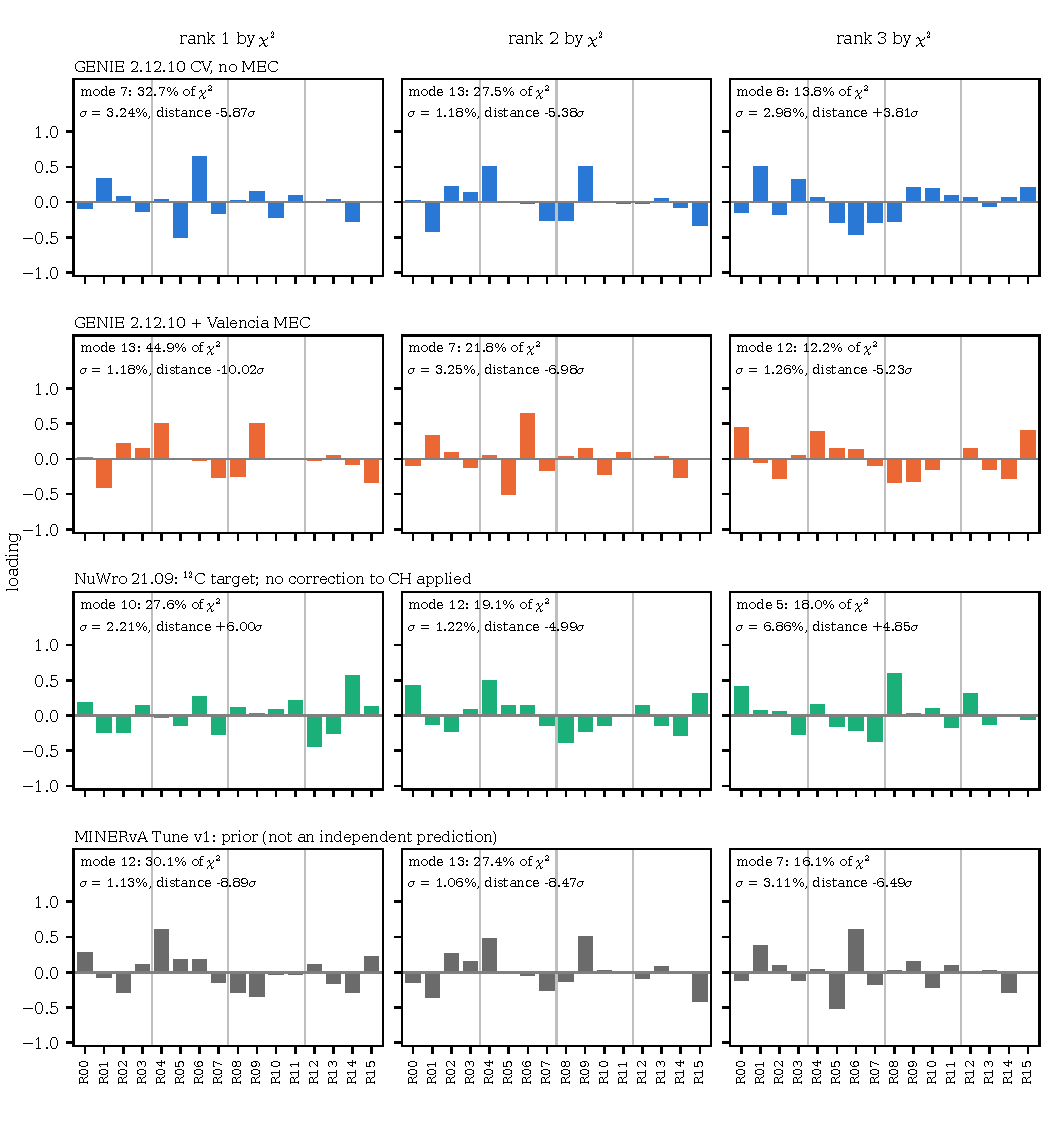
\includegraphics[width=\linewidth]{figures/fd_g_fig_modes.pdf}
\caption{The three eigenmodes that carry the largest shares of each sixteen-cell prediction's $\chi^2$ (columns, by rank), for GENIE CV, GENIE + MEC, NuWro and MINERvA Tune~v1 (rows), from the reported comparison on $C_{\mathrm{total}}+C_{\mathrm{resp}}+V_g$ relative to $f$. The bars are each mode's unit loadings on R00--R15, signed so that the largest loading is positive. Each panel gives the mode's share of the $\chi^2$, its relative $\sigma$ and the prediction's distance along it, the projection over $\sigma$. The residual is $(f-g)/f$, so a positive distance means that the data lie above the prediction along the mode as signed. GiBUU, compared on 8 cells, has no modes here.}
\label{fig:fived16-modes}
\end{figure}

\begin{table}[htbp]
\centering\footnotesize
\caption{Eigenmode breakdown of the reported $\chi^2$: the fewest modes, in $\chi^2$ order, carrying \fvval{diag-fractions}\,\% of it, and the top mode's share of the $\chi^2$, its relative $\sigma$ and its dominant block.}
\label{tab:fived16-diag}
\begin{tabular}{@{}lcccrrl@{}}
\toprule
prediction & \multicolumn{3}{c}{modes for \fvval{diag-fractions}\,\%} & top mode (\% of $\chi^2$) & $\sigma$ (\%) & block \\
\midrule
\fvval{label-gcv} & \fvval{diag-gcv-reported-modes50} & \fvval{diag-gcv-reported-modes90} & \fvval{diag-gcv-reported-modes99} & \fvval{diag-gcv-reported-top-share} & \fvval{diag-gcv-reported-top-sigma} & \fvval{diag-gcv-reported-top-block} \\
\fvval{label-gmec} & \fvval{diag-gmec-reported-modes50} & \fvval{diag-gmec-reported-modes90} & \fvval{diag-gmec-reported-modes99} & \fvval{diag-gmec-reported-top-share} & \fvval{diag-gmec-reported-top-sigma} & \fvval{diag-gmec-reported-top-block} \\
\fvval{label-nuwro} & \fvval{diag-nuwro-reported-modes50} & \fvval{diag-nuwro-reported-modes90} & \fvval{diag-nuwro-reported-modes99} & \fvval{diag-nuwro-reported-top-share} & \fvval{diag-nuwro-reported-top-sigma} & \fvval{diag-nuwro-reported-top-block} \\
\fvval{label-gibuu} & \fvval{diag-gibuu-reported-modes50} & \fvval{diag-gibuu-reported-modes90} & \fvval{diag-gibuu-reported-modes99} & \fvval{diag-gibuu-reported-top-share} & \fvval{diag-gibuu-reported-top-sigma} & \fvval{diag-gibuu-reported-top-block} \\
\fvval{label-tune} & \fvval{diag-tune-reported-modes50} & \fvval{diag-tune-reported-modes90} & \fvval{diag-tune-reported-modes99} & \fvval{diag-tune-reported-top-share} & \fvval{diag-tune-reported-top-sigma} & \fvval{diag-tune-reported-top-block} \\
\bottomrule
\end{tabular}
\end{table}

Cell R04 ($\pT<\fvval{h2-mid-pt}$, $\pPar\geq\fvval{h2-mid-pz}$, $\Eavail<\fvval{h2-mid-eavail}$, $q_3<\fvval{h2-mid-q3}$) has the smallest relative $\sigma$ of the sixteen, \fvval{r04-sigma-total}\,\%, of which flux is the largest group at \fvval{r04-sigma-flux}\,\%. Under the flux block alone its correlation with the \fvval{r04-ncorr} cells that load with it in the top modes is \fvval{r04-corrflux-min}--\fvval{r04-corrflux-max}; under the reported covariance it is \fvval{r04-corr-min}--\fvval{r04-corr-max}.

